\chapter{Summary and Discussion of Results}
\label{chapterlabel5}

In this chapter, some experiments are implemented to show the results of theory discussed in the previous chapters. We will gives the experimental results and compare different methods. The discussion covers the advantage and disadvantage of the techniques. Also, after this procedure, we do some simulations on RTB. 

To evaluate the performance of a predictor, a number of reasonable machine learning measures are developed such as log-likelihood of test data or the area under the receiver-operator curve (AUC). In the experiment, we use 2-class logarithmic loss
\begin{equation}
logloss = -\frac{1}{L}\sum_{i=1}^{L}y_i \log \bar{y}_i+(1-y_i) \log (1-\bar{y}_i)
\end{equation}
where $L$ is the total number of instances, $y_i$ is the binary label (0 or 1) and $\bar{y}_i$ is the predicted click probability of impressions. We also apply K-fold cross-validation to calculate the mean logloss which can represent the overall error of estimation.

Besides, Area-Under-ROC (AUC) is also a pretty good metric for measuring ranking quality without considering calibration. ROC curves are typically used in binary classification. The two axises are True positive rate and False positive rate respectively
\begin{center}
$\text{True positive} = \frac{\sum \text{True positve}}{\sum \text{Condition positive}}$, 
$\text{False positive} = \frac{\sum \text{False positive}}{\sum \text{Condition negative}}$.
\end{center}
It is ideal to maximize the true positive rate while minimizing the false positive rate. We use the full dataset to train the model and evaluate the performance.

We do not consider the features Bid ID, Log Type, iPinYou ID, URL, URL ID, Bidding Price, Paying Price, Key Page URL because they are almost unique and not repeated for each instance. The uniqueness is meaningless for CTR prediction. GBDT with depth 7 is used to generate 10 categorical features for each bid request feature. We use $\alpha=0.1$ and $\beta=1.0$ for FTRL-proximal and FFM model. Our final model is an ensemble of the three models. 

\begin{table}[H]
\caption{The logloss of CTR estimation performance}
\label{tab:CTR AUC}
\begin{center}
\begin{tabular}{ l l l l l l } 
\hline
Advertiser ID & Season & BOPR & FTRL & FFM & Ensemble \\
\hline
1458 & 2 & 0.00162 & 0.00156 & 0.00154 & 0.00153 \\
2259 & 3 & 0.00285 & 0.00274 & 0.00275 & 0.00272 \\
2261 & 3 & 0.00256 & 0.00256 & 0.00256 & 0.00256 \\
2821 & 3 & 0.00490 & 0.00489 & 0.00482 & 0.00485 \\
2997 & 3 & 0.02321 & 0.02293 & 0.02273 & 0.02277 \\
3358 & 2 & 0.00273 & 0.00268 & 0.00270 & 0.00260 \\
3386 & 2 & 0.00615 & 0.00599 & 0.00597 & 0.00590 \\
3427 & 2 & 0.00241 & 0.00237 & 0.00219 & 0.00208 \\
3476 & 2 & 0.00258 & 0.00249 & 0.00253 & 0.00248 \\
Total & 2,3 & 0.00221 & 0.00229 & 0.00211 & 0.00216 \\
\hline
\end{tabular}
\end{center}
\end {table}

The logloss metric gives the similar result as AUC. However, logloss might not show the importance of relative information gain. It may have divergence bias in it.

\begin{table}[H]
\caption{The AUC of CTR estimation performance}
\label{tab:CTR AUC}
\begin{center}
\begin{tabular}{ l l l l l l } 
\hline
Advertiser ID & Season & BOPR & FTRL & FFM & Ensemble \\
\hline
1458 & 2 & 0.9881 & 0.9887 & 0.9901 & 0.9915 \\
2259 & 3 & 0.6880 & 0.6934 & 0.6996 & 0.7002 \\
2261 & 3 & 0.6265 & 0.6270 & 0.6239 & 0.6295 \\
2821 & 3 & 0.6071 & 0.6097 & 0.6009 & 0.6131 \\
2997 & 3 & 0.6031 & 0.6010 & 0.5834 & 0.5837 \\
3358 & 2 & 0.9759 & 0.9786 & 0.9821 & 0.9815 \\
3386 & 2 & 0.7928 & 0.7908 & 0.7909 & 0.7922 \\
3427 & 2 & 0.9776 & 0.9820 & 0.9832 & 0.9869 \\
3476 & 2 & 0.9675 & 0.9721 & 0.9701 & 0.9768 \\
Total & 2,3 & 0.8554 & 0.8604 & 0.8620 & 0.8680 \\
\hline
\end{tabular}
\end{center}
\end {table}

\begin{figure}[htbp]

\begin{subfigure}{0.5\textwidth}
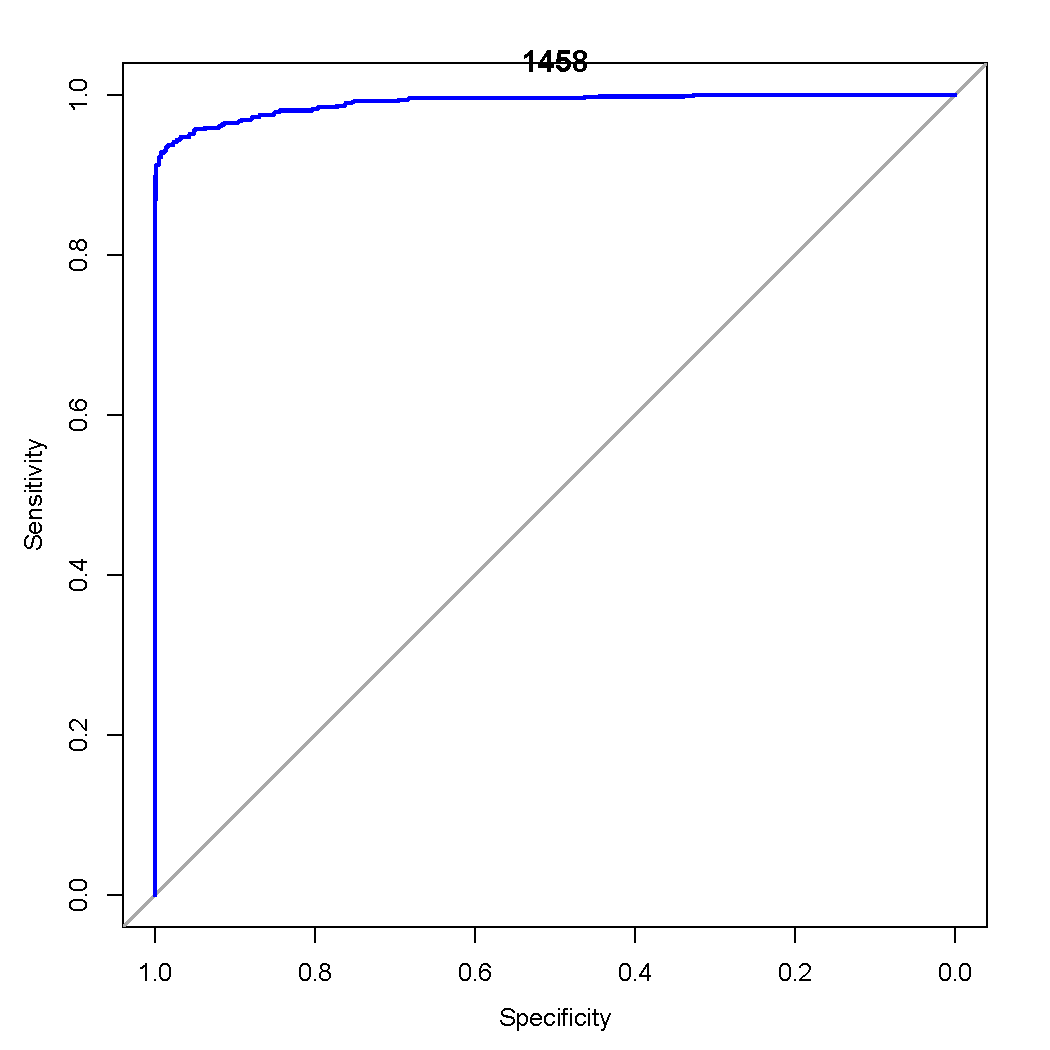
\includegraphics[width=0.9\linewidth, height=5cm]{1458.pdf}
\caption{1458}
\label{fig:sub1}
\end{subfigure}
\begin{subfigure}{0.5\textwidth}
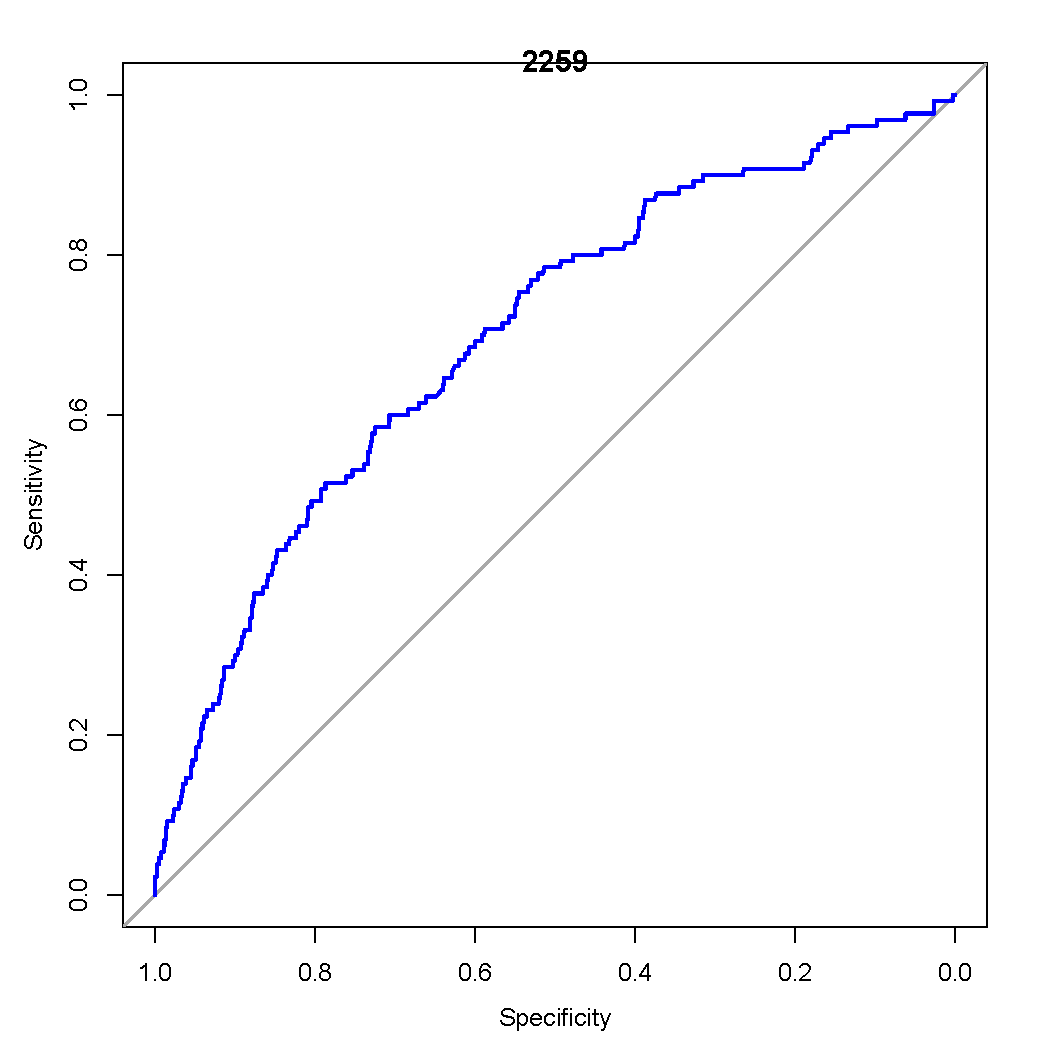
\includegraphics[width=0.9\linewidth, height=5cm]{2259.pdf}
\caption{2259}
\label{fig:2259}
\end{subfigure}
\begin{subfigure}{0.5\textwidth}
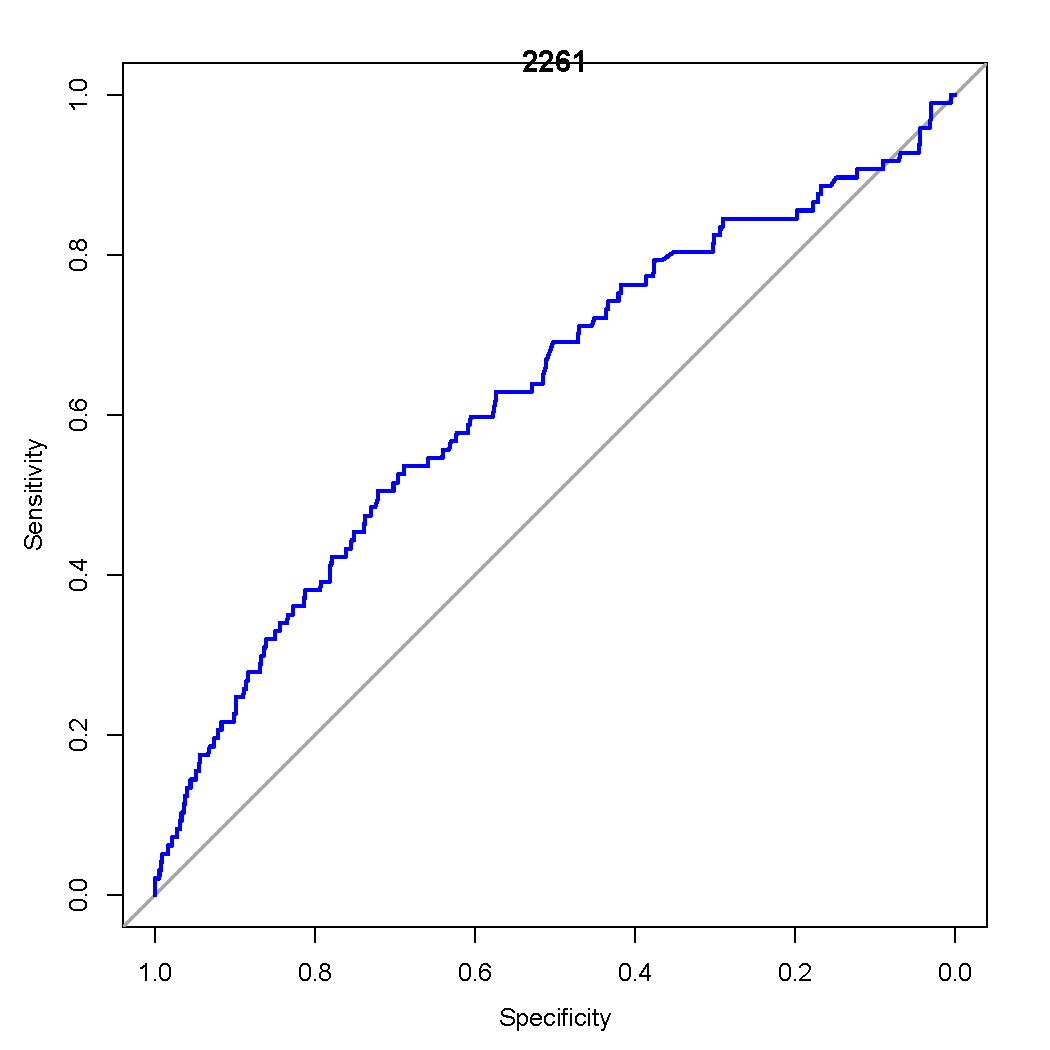
\includegraphics[width=0.9\linewidth, height=5cm]{2261.pdf}
\caption{2261}
\label{fig:2261}
\end{subfigure}
\begin{subfigure}{0.5\textwidth}
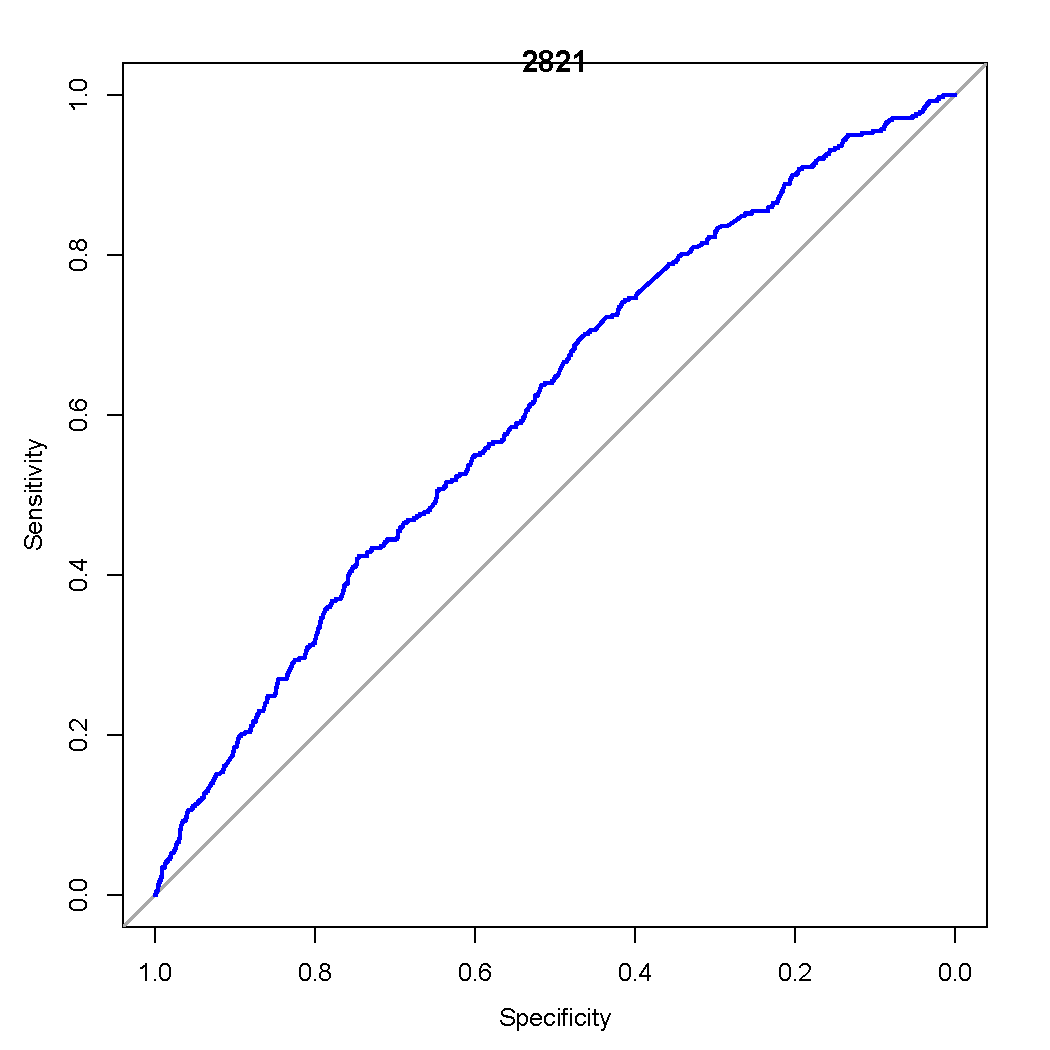
\includegraphics[width=0.9\linewidth, height=5cm]{2821.pdf}
\caption{2821}
\label{fig:2821}
\end{subfigure}
\begin{subfigure}{0.5\textwidth}
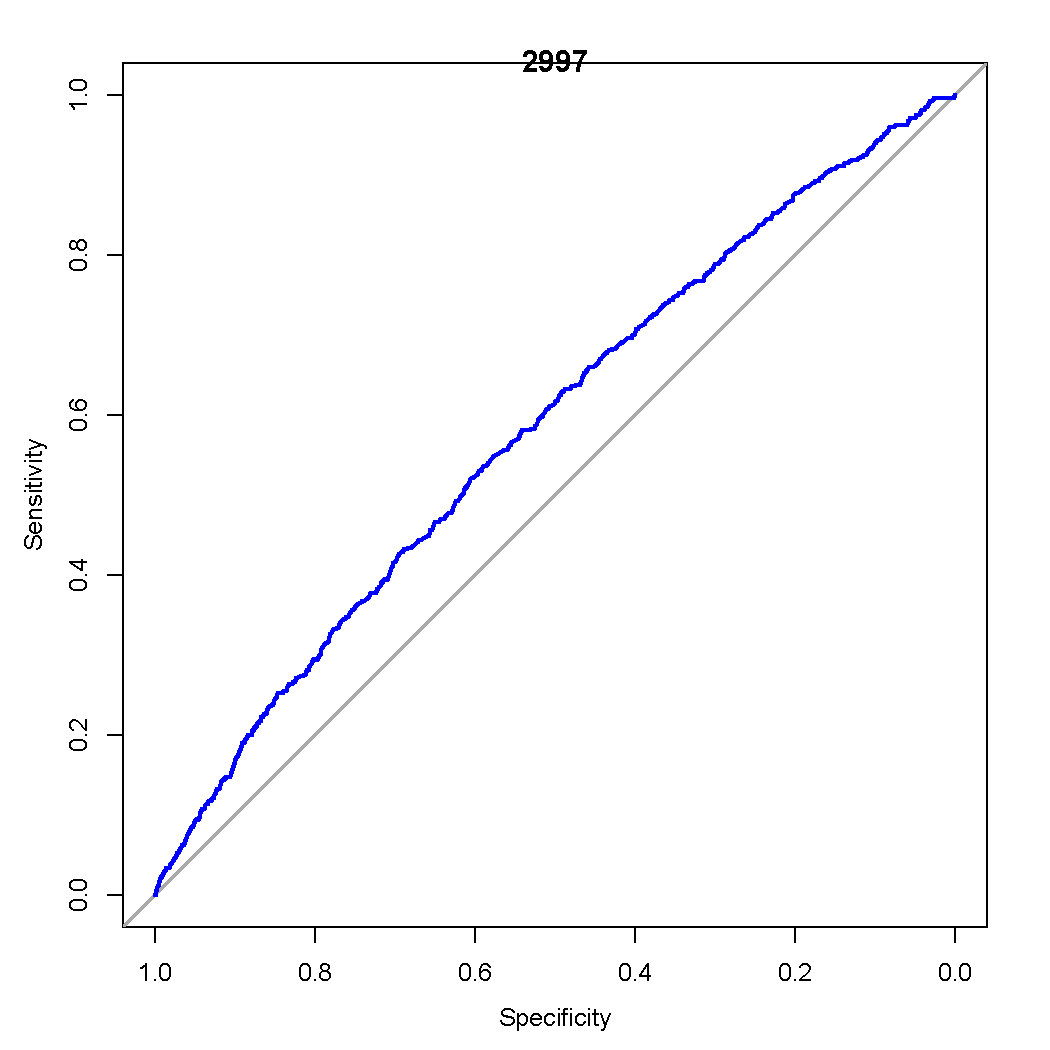
\includegraphics[width=0.9\linewidth, height=5cm]{2997.pdf}
\caption{2997}
\label{fig:2997}
\end{subfigure}
\begin{subfigure}{0.5\textwidth}
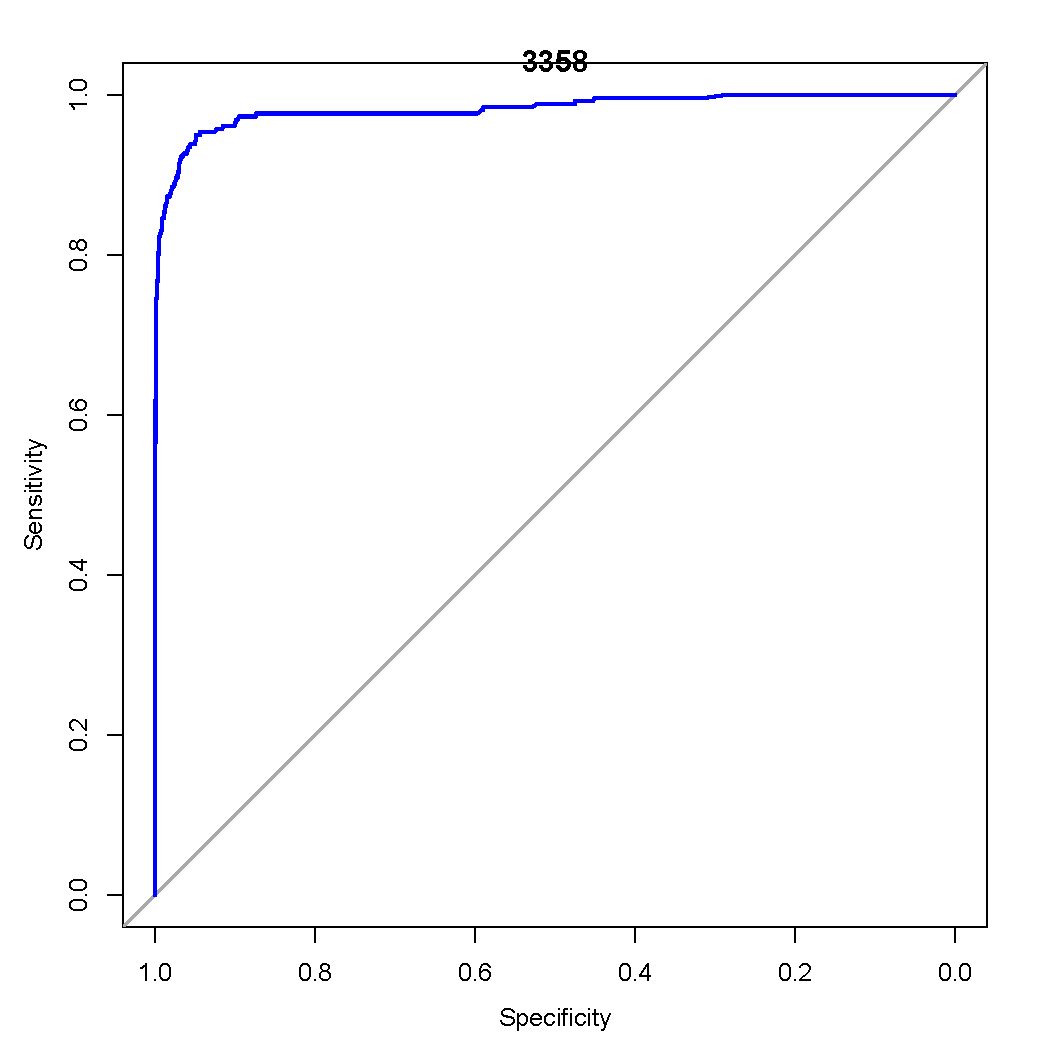
\includegraphics[width=0.9\linewidth, height=5cm]{3358.pdf}
\caption{3358}
\label{fig:3358}
\end{subfigure}
\begin{subfigure}{0.5\textwidth}
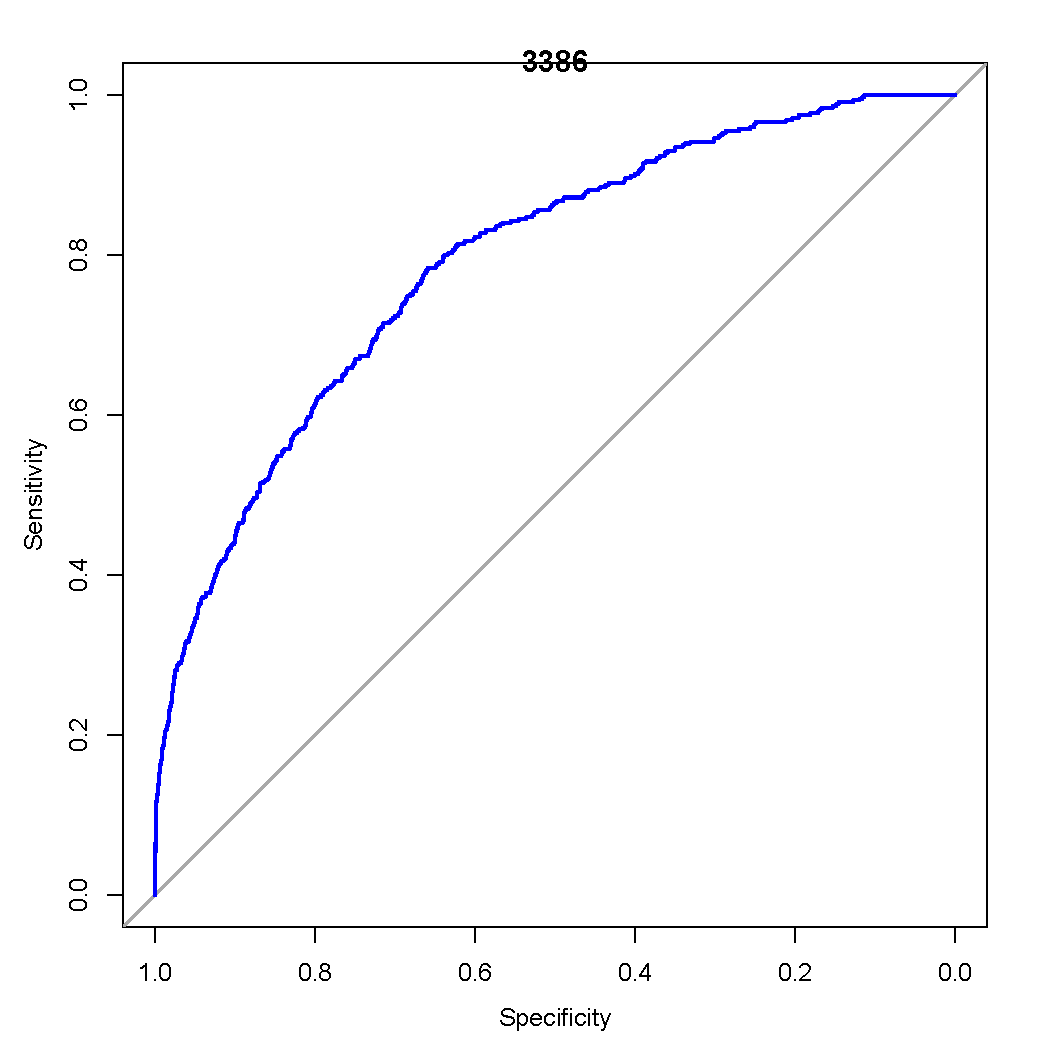
\includegraphics[width=0.9\linewidth, height=5cm]{3386.pdf}
\caption{3386}
\label{fig:3386}
\end{subfigure}
 \begin{subfigure}{0.5\textwidth}
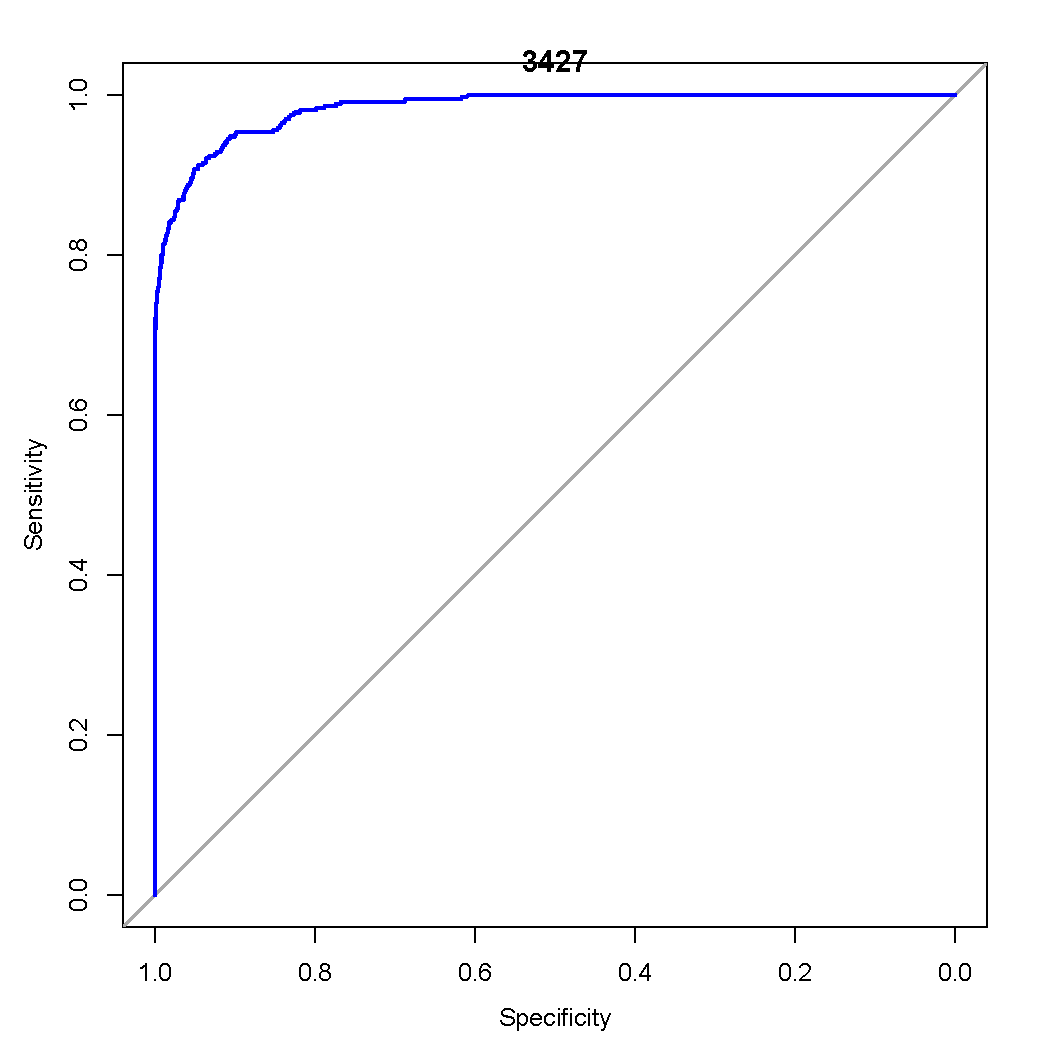
\includegraphics[width=0.9\linewidth, height=5cm]{3427.pdf}
\caption{3427}
\label{fig:3427}
\end{subfigure}

\label{fig:image1}
\end{figure}

\begin{figure}[htbp]

\begin{subfigure}{0.5\textwidth}
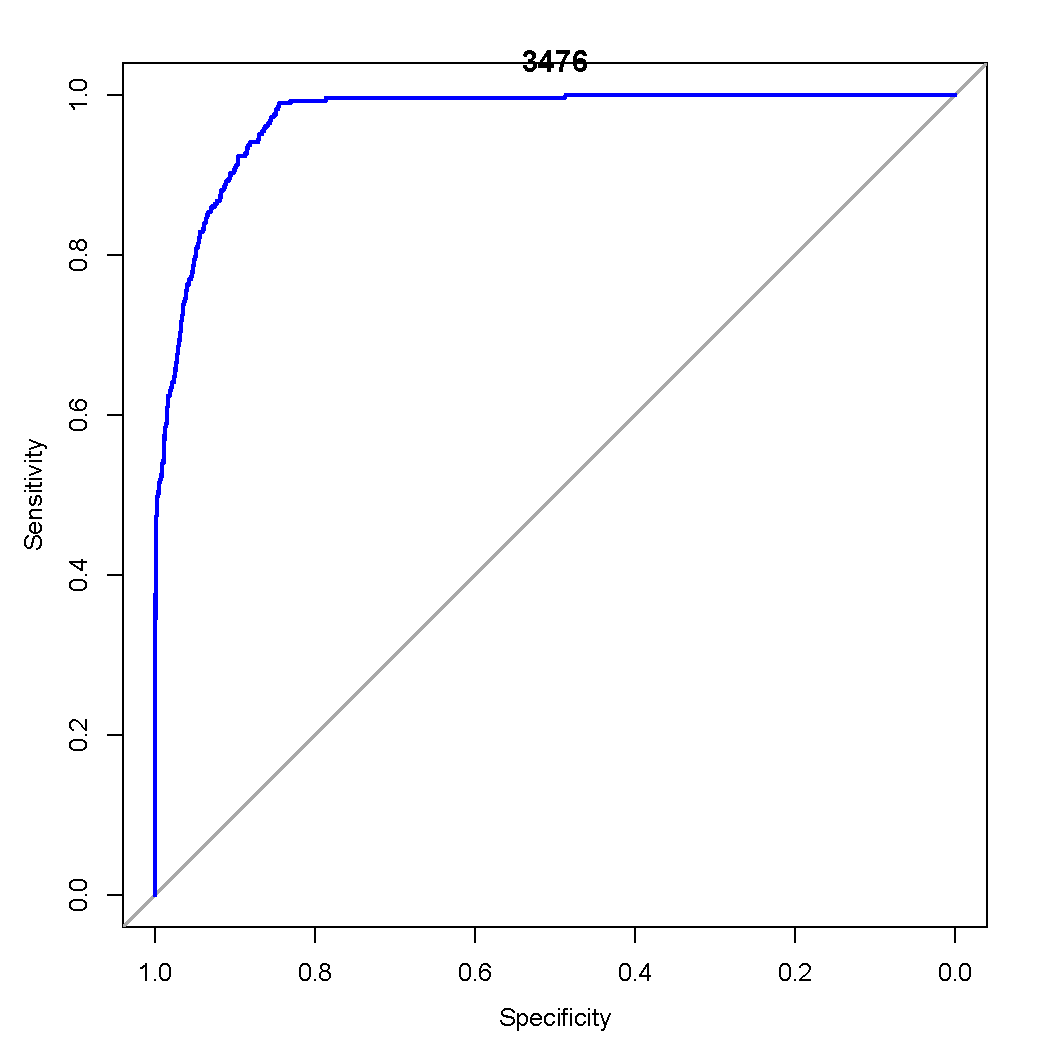
\includegraphics[width=0.9\linewidth, height=5cm]{3476.pdf}
\caption{3476}
\label{fig:3476}
\end{subfigure}
\begin{subfigure}{0.5\textwidth}
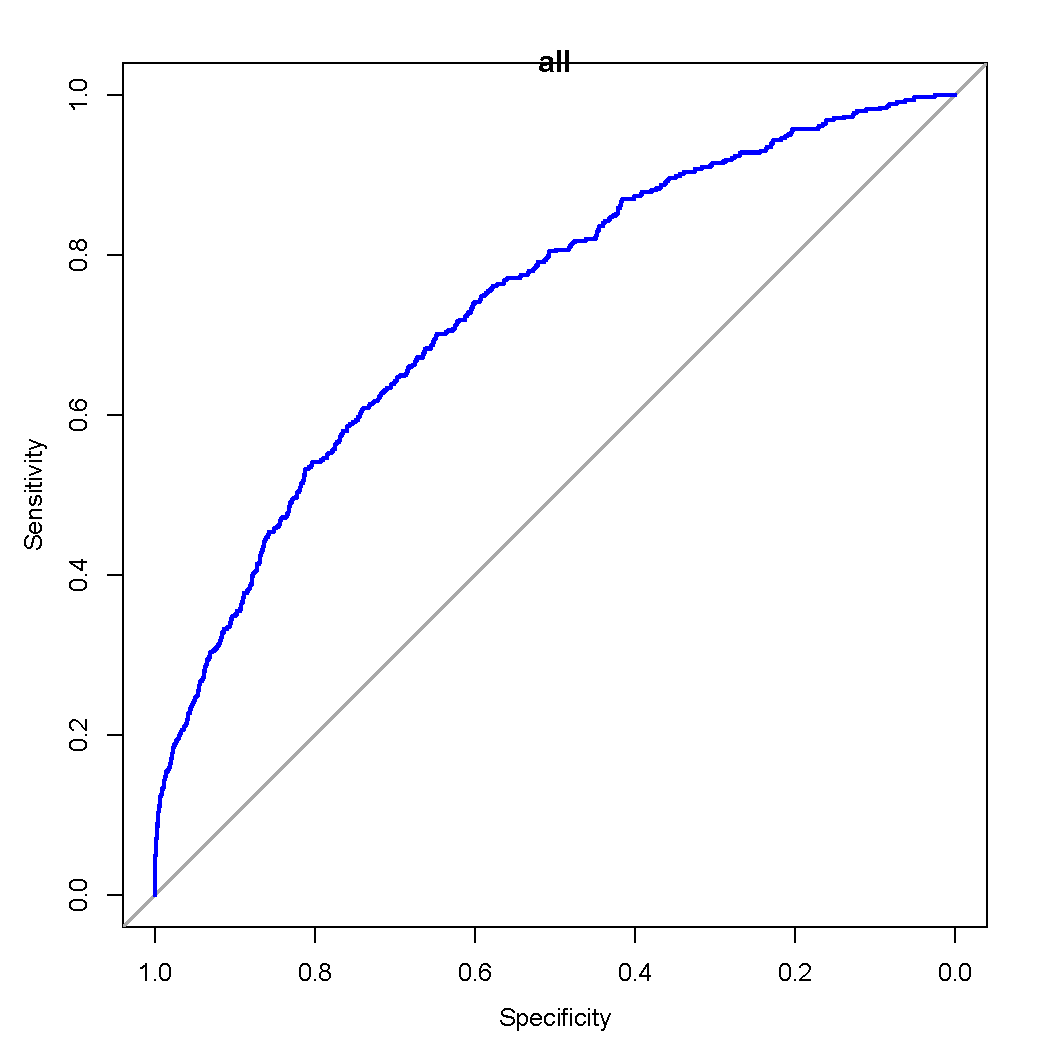
\includegraphics[width=0.9\linewidth, height=5cm]{all.pdf}
\caption{Total}
\label{fig:all}
\end{subfigure}

\caption{The ROC metric for evaluating the ensemble CTR output quality of advertisers}
\label{fig:image2}
\end{figure}

For the most of time, FFM gives outperformance. The result of FTRL-Proximal and FFM is very similar as they are based on the similar optimization objective except the lasso term, but they find the weights through different approaches. FTRL-Proximal, which ends up being comparable in performance with BOPR, and performs better than all other LR SGD schemes.

According to the benchmark \cite{zhang2014real}, transforming real-valued input features with boosted decision trees significantly increases the prediction performance of probabilistic linear classifiers. This motivates a hybrid model architecture that concatenates boosted decision trees and a sparse linear classifier.

As we can see from the AUC of ensemble results, we find that the AUC performance increases by 1$\%$-5$\%$ after ensemble. The Figure~\ref{fig:image2} is the ROC metric for evaluating the ensemble CTR output quality of advertisers.

One more thing we need to take into consideration is the effect of imbalanced ratio. When referring to Table~\ref{tab:Advertiser}, the percentage of clicked instances is very low. By some subsampling tricks, we can identify the influence of imbalanced ratio according to Figure~\ref{fig:imbalance}. The x-axis represents the percentage value and y-axis is the corresponding AUC. After the imbalanced ratio reaches a certain percentage (0.2$\%$), the AUC turns to become steady.

\begin{figure}[htbp]
\centering
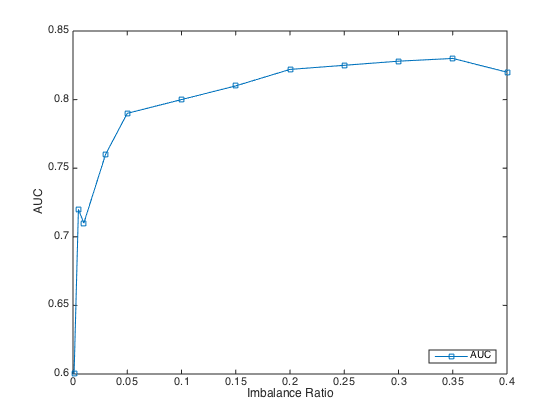
\includegraphics[width=0.8\textwidth]{imbalance.png}
\caption{The influence of the imbalance ratio on learning performance}
\label{fig:imbalance}
\end{figure}

In practical application, we should keep data fresh. It is worth retraining at least daily. In this thesis, we use the full dataset as data is limited.

In terms of reinforcement learning experiments, we cannot use the origin dataset because it is too large to implement as a dynamic programming process. We generate an ideal ad feature but it only contains 10 binary elements. Also, the total impression is given by $T=5000$ and set the learning rate $\epsilon=0.05$. If Q table is converged, the learning process will terminate. We show the first 200 winning bids in Figure \ref{fig:Q} and Figure \ref{fig:S}. 

We only plot the winning bids because feedback only can be observed from them. We find the performance of Q-Leanring and Sarsa is very similar, except that Sarsa shows a high divergence when the number of iterations is small. However, when the number of iterations is large enough and learning process is converged, Q-Learning and Sarsa shows the same outcome. 

The computational results are almost the same with the conclusion of Kernelized Value Function Approximation. Advertisers are willing to bid a higher price than their true value in the very beginning of the sequential auctions. The sacrifice of current utility is for the exploration of market price landscape. When the number of remaining impressions is quite small, they turn to bid their true value and it becomes one-shot auction with side information in the end.
\begin{figure}[htbp]

\begin{subfigure}{0.5\textwidth}
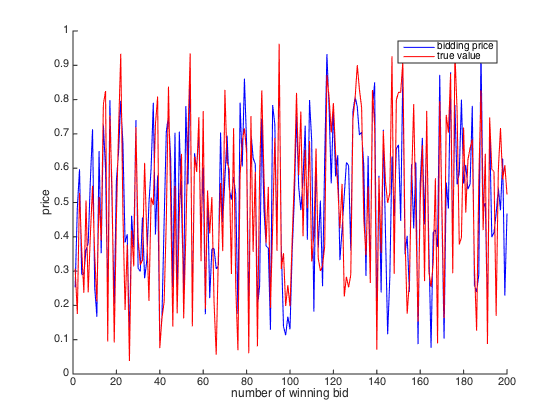
\includegraphics[width=0.9\linewidth, height=5cm]{Q100.png}
\caption{100 iterations}
\label{fig:Q100}
\end{subfigure}
\begin{subfigure}{0.5\textwidth}
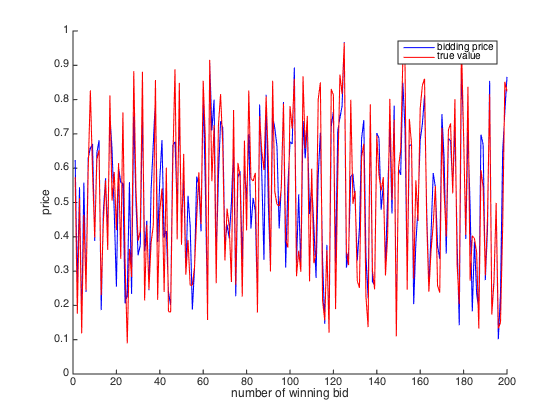
\includegraphics[width=0.9\linewidth, height=5cm]{Q200.png}
\caption{200 iterations}
\label{fig:Q200}
\end{subfigure}
\begin{subfigure}{0.5\textwidth}
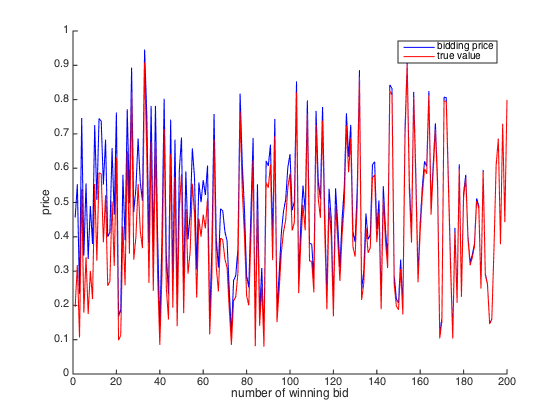
\includegraphics[width=0.9\linewidth, height=5cm]{Q300.png}
\caption{300 iterations}
\label{fig:Q300}
\end{subfigure}
\begin{subfigure}{0.5\textwidth}
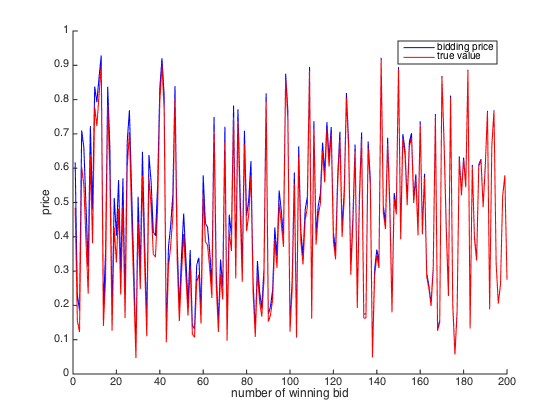
\includegraphics[width=0.9\linewidth, height=5cm]{Q400.png}
\caption{400 iterations}
\label{fig:Q400}
\end{subfigure}

\caption{The number of winning bid and price for various iterations of Q-Learning}
\label{fig:Q}
\end{figure}

\begin{figure}[htbp]

\begin{subfigure}{0.5\textwidth}
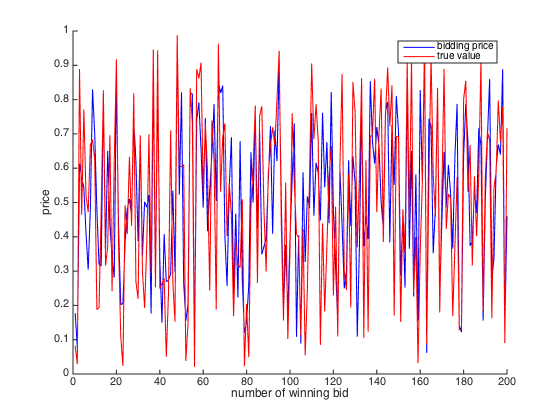
\includegraphics[width=0.9\linewidth, height=5cm]{S100.png}
\caption{100 iterations}
\label{fig:S100}
\end{subfigure}
\begin{subfigure}{0.5\textwidth}
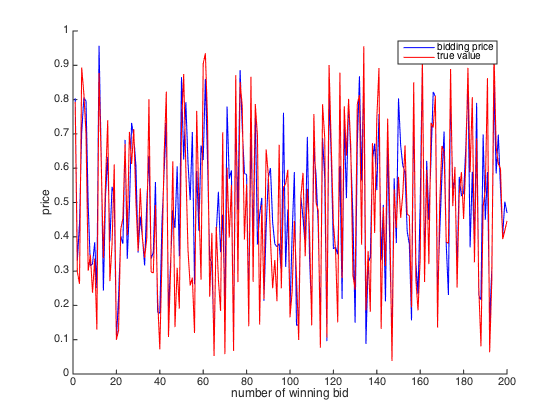
\includegraphics[width=0.9\linewidth, height=5cm]{S200.png}
\caption{200 iterations}
\label{fig:S200}
\end{subfigure}
\begin{subfigure}{0.5\textwidth}
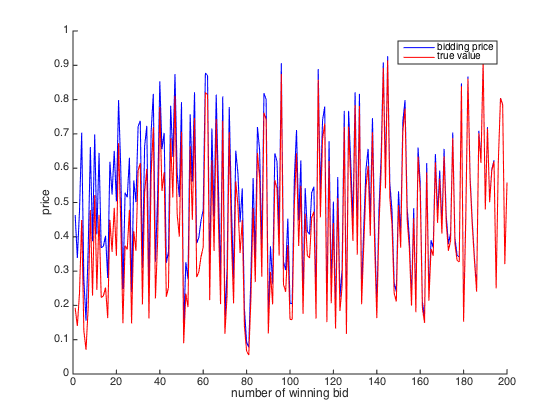
\includegraphics[width=0.9\linewidth, height=5cm]{S300.png}
\caption{300 iterations}
\label{fig:S300}
\end{subfigure}
\begin{subfigure}{0.5\textwidth}
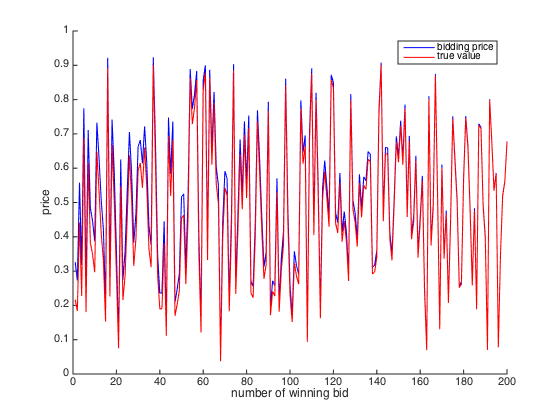
\includegraphics[width=0.9\linewidth, height=5cm]{S400.png}
\caption{400 iterations}
\label{fig:S400}
\end{subfigure}

\caption{The number of winning bid and price for various iterations of Sarsa}
\label{fig:S}
\end{figure}





